\documentclass[a4paper, 12pt]{amsart}

\linespread{1.3}

% \usepackage{studia}
\usepackage{graphicx}
\usepackage{url}
\usepackage{listings}
\usepackage{algorithm}
\usepackage{algorithmic}
\usepackage{wrapfig}
\usepackage{lscape}
\usepackage{rotating}
\usepackage{epstopdf}

\setcounter{page}{1}
% \coordinates{..}{..}{2015}

\title[Reflecta]{Reflecta - An open-source framework for motion capture acquisition} % Short Title and Title

\author{Alexandru Marinescu}
\address{Dept. of Computer Science, Babe\c{s}-Bolyai University, Kog\u{a}lniceanu 1, 400084 Cluj-Napoca, Romania}
\email{mais0856@scs.ubbcluj.ro}
\date{June 1, 2015} % Submission Date

% AMS Subject Classification (2010)
% http://www.ams.org/mathscinet/msc/msc2010.html
% 68-00 General reference works (handbooks, dictionaries, bibliographies, etc.)
% 68-01 Instructional exposition (textbooks, tutorial papers, etc.)
% 68-02 Research exposition (monographs, survey articles)
% 68-03 Historical (must also be assigned at least one classification number from Section 01)
% 68-04 Explicit machine computation and programs (not the theory of computation or programming)
% 68-06 Proceedings, conferences, collections, etc.
% Specific categories:
% 68U05 Computer graphics; computational geometry [See also 65D18]
% 68T05 Learning and adaptive systems [See also 68Q32, 91E40]
% 92B20 Neural networks, artificial life and related topics [See also 68T05, 82C32, 94Cxx]
\subjclass[2010]{68U05}

% ACM Computing Classification System (1998)
% http://www.acm.org/about/class/1998
% CODE Chapter [\textbf{Topic}]: Subtopic -- \textit{Detail};
% \subjclassCR
% {
% A.1 General Literature [\textbf{INTRODUCTORY AND SURVEY}];
% I.3.7 Computing Methodologies [\textbf{COMPUTER GRAPHICS}]: Three-Dimensional Graphics and Realism -- \textit{Animation}
% }

\keywords{Kinect, body joints, facial expressions, animation, avatars, noise reduction}

\begin{document}

\begin{abstract}
We wish to provide insight into the inner workings of Reflecta - our framework for motion capture data acquisition using the Microsoft Kinect for Windows v2 sensor and interoperating with the Unity 5 game engine. Taking into account the rapid development in the field of Natural User Interface (NUI) enabled applications, we felt that we could augment existing, state of the art hardware sensors with a comprehensive solution for processing the sensor input and converting it into actual, meaningful animation data. We have decided to explore this niche in the industry which, at the time of this writing lacks a free, open-source alternative. Currently, our proposed solution handles facial expression and joint orientation data, providing fully configurable filtering algorithms for reducing input noise, and is capable of outputting either raw data, animation clips used natively by the Unity game engine or BVH (BioVision Hierarchy), ready to import in the most widely used 3D modelling software. We have strived to make Reflecta as loosely-coupled as possible and have outlined the difficulties encountered together with our proposed solutions. The range of applications for Reflecta is virtually limitless, from helping indie game developers reach their goal to aiding medical recovery for disabled patients.
\end{abstract}

\maketitle

\clearpage

\tableofcontents

\clearpage

\section{Introduction}

\subsection{What is Reflecta?}

\begin{figure}[htb]
\centering
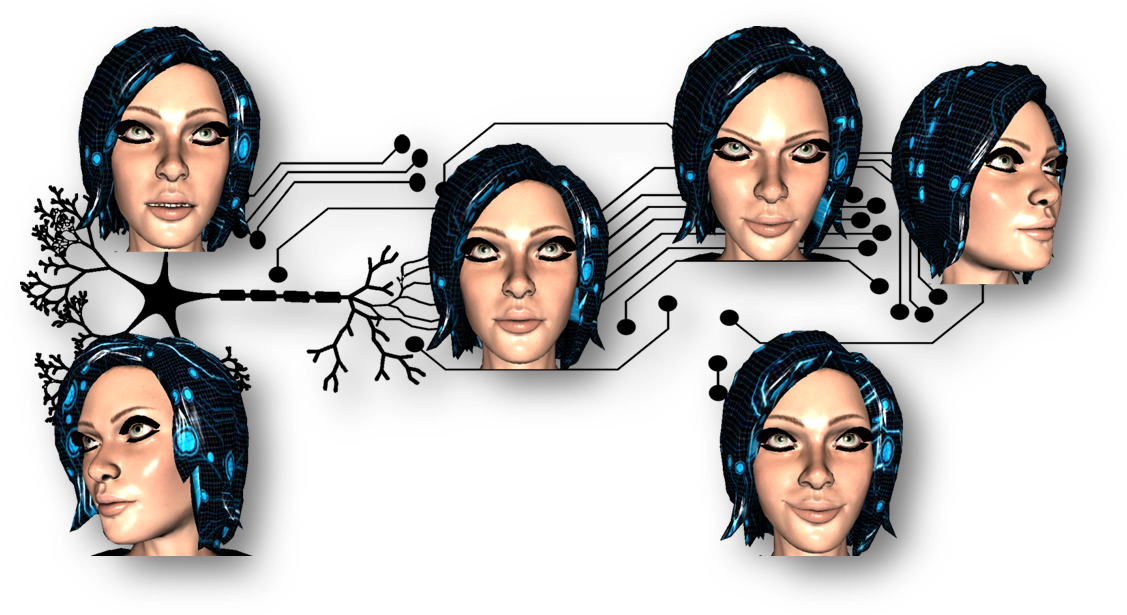
\includegraphics[width=.9\linewidth]{fig_reflecta_splash}
\caption{Reflecta range of expressions.}
\label{fig:reflecta_splash}
\end{figure}

Reflecta (Figure \ref{fig:reflecta_splash}) is a small but powerful framework which enables users owning a Kinect for Windows v2 sensor to record raw motion capture data (mocap) in our internal format (distinguished by the ``.mocap'' file extension) and provides real-time visualization of the tracked individual by means of a 3D avatar. Basically, the user can view a ``reflection'' of himself as seen by the sensor, rendered within a 3D graphical environment (hence the name of the project). Reflecta was initially designed for high-definition facial expression tracking, by mapping internally between the expression weights from the Kinect sensor (input) to the facial blend shapes from the Mixamo rigged model (output).

Shortly afterwards, it was extended to support mimicking the joint positions and orientations applied a Unity Mecanim-enabled model (which was also generated from Mixamo's Fuse content creator, but any Mecanim compatible model should suffice). A wizard utility is bundled within the framework that converts recorded raw mocap data to Unity's own animation clips, which can then be simply dragged and dropped on the rigged model and used as any regular animation in game.

We decided to take our project one step further and implement export capabilities to the industry standard humanoid animation format, namely BioVision Hierarchy (or BVH). BVH is a textual, human readable format for specifying animations for biped/humanoid models \cite{bib_motion_capture_explained, bib_motion_capture_computer_animation, bib_motion_capture_editing}. It is composed of 2 sections: the bone hierarchy specification and the actual animation keyframe values. This decision helps integrate Reflecta into the workflow of existing, industry standard 3D modelling software such as 3ds Max \cite{bib_3ds_max}, Maya \cite{bib_maya}, or Blender \cite{bib_blender}.

\subsection{The incentive of the project}

The authors want to lay the foundations for an open-source, flexible tool targeted at indie/hobbyist game developers who lack 3D modelling and animation expertise, by effectively giving them the ability to record their own motion capture data. The most up-to-date source code for Reflecta can be found on GitHub at: \url{https://github.com/Zerseu/Reflecta}. The reader will find documented below the actual reasons we decided to take this path:

\begin{itemize}
\item Existing tools are either very expensive for indie developers (take Poser Pro GameDev for example \cite{bib_poser}) or lack certain features;
\item Our proposed solution takes into consideration both body joint orientations and facial expression morphs in order to fully exploit the Kinect sensor hardware capabilities;
\item It frees artists from the burden of creating animation clips for 3D models and allows them to focus on more important tasks;
\item Fully integrates with one of the most widely used game engines - Unity 5 and has full support for Mixamo rigged models;
\item Nevertheless, Reflecta can be employed to animate any 3D model that provides a basic Mecanim bone hierarchy and facial blend shapes with none to minimal modifications to the underlying code;
\item Speech synthesis and recognition support, which opens up virtually infinite scenarios of usage in the NUI field of application;
\item Wizard to convert mocap data to Unity animation clips;
\item Possibility to export mocap data to industry standard formats such as BVH;
\item Fully configurable filtering algorithms for advanced reduction of input noise, which is inherent to all hardware sensors;
\end{itemize}

\subsection{Structure of this paper}

The paper is divided into 9 sections, each containing relevant subsections for the topics discussed.

The first section outlines the motives behind creating this framework. Next, we acquaint the reader with the concept of motion capture acquisition and existing technologies. Section 3 is an in depth analysis of the architecture we have chosen and its benefits, while sections 4 to 6 explore the techniques we applied to handle body, facial expression and noise, respectively.

Finally we reach a conclusion regarding our solution and provide the reader with some relevant future directions of improvement.

\subsection{The author's contribution}

We would like to emphasize the author's original contribution to existing literature. To begin with, at the time this article was written, there was no open-source framework or solution that takes into account both body and facial input data. Furthermore, existing partial solutions provide obscure mappings between different animation systems (as a concrete example, we have seen implementations that did not handle input in a unified way). This unification of the input pipeline is a defining feature of our solution.

As an addition, we have designed DESP (double-exponential smoothing) predictors and applied custom noise-reduction algorithms for the following inputs: facial blend weights (floating point type, DESP, average and power function), joint positions (Vector3 type, DESP and average) and joint orientations (Quaternion, DESP and average with our custom implementation because the algorithm suggested in original paper had discontinuities on specific rotations).

\clearpage

\section{Motion capture in detail}

\begin{figure}[htb]
\centering
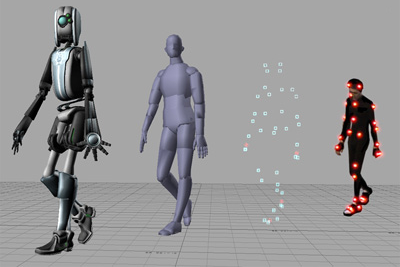
\includegraphics[width=.9\linewidth]{fig_motion_capture}
\caption{From motion capture to character animation.}
\label{fig:motion_capture}
\end{figure}

The concept of motion capture is not new; it has been around for quite some time. An example of an early form of motion capture is the film ``Snow White and the Seven Dwarfs'' (1937), where actors and actresses would act out scenes and would be filmed. Afterwards, the animators used the actual footage as guide lines for drawing the characters. ``Final Fantasy: The Spirits Within'' (2001) was the first widely released movie to be made primarily with motion capture technology. Despite its poor box-office intake, supporters of motion capture technology became aware of its usefulness. Motion capture is used extensively in modern games and movies in order to add an extra amount of realism to CGI imagery (Figure \ref{fig:motion_capture}), mainly because the complex body muscle and bone interactions are still difficult to compute even on large scale render stations. For video games, the earliest application of motion capture was the arcade game ``Virtua Fighter 2'' (1994). Below we give a list of some advantages and drawbacks of motion capture acquisition.

Advantages:

\begin{itemize}
\item More rapid, even real time results can be obtained. In entertainment applications this can reduce the costs of keyframe-based animation;
\item The amount of work does not vary with the complexity or length of the performance to the same degree as when using traditional techniques. This allows many tests to be done with different styles or deliveries, giving a different personality only limited by the talent of the actor;
\item Complex movement and realistic physical interactions such as secondary motions, weight and exchange of forces can be easily recreated in a physically accurate manner;
\item The amount of animation data that can be produced within the given time is extremely large when compared to traditional animation techniques. This contributes to both cost effectiveness and meeting production deadlines;
\item Potential for free software and third party solutions reducing costs;
\end{itemize}

Disadvantages:

\begin{itemize}
\item Specific hardware and special software programs are required to obtain and process the data;
\item The cost of the software, equipment and personnel required can be prohibitive for small productions;
\item The capture system may have specific requirements for the space it is operated in, depending on camera field of view;
\item When problems occur, it is easier to re-shoot the scene rather than trying to manipulate the data. Only a few systems allow real time viewing of the data to decide if the take needs to be redone;
\item The initial results are limited to what can be performed within the capture volume without extra editing of the data;
\item Movement that does not follow the laws of physics cannot be captured;
\item If the computer model has different proportions from the capture subject, artefacts may occur. For example, if a cartoon character has large, over-sized hands, these may intersect the character's body if the human performer is not careful with their physical motion;
\end{itemize}

Only recently has motion capture become available to the average consumer with the introduction of hardware sensors which can easily be interfaced by means of an API.

\subsection{Dedicated hardware sensors}

This section represents a case study of existing consumer-grade hardware sensors and their suitability to our purpose.

\begin{figure}[htb]
\centering
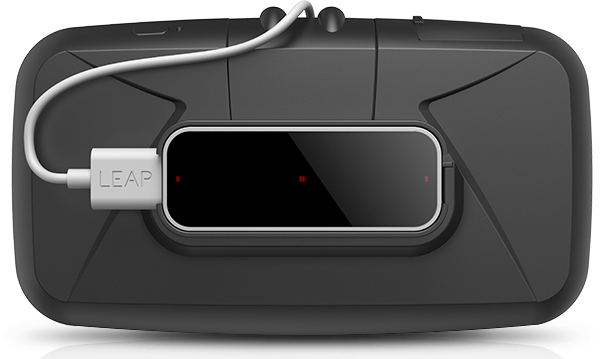
\includegraphics[width=.9\linewidth]{fig_leap_motion}
\caption{The Leap Motion sensor.}
\label{fig:leap_motion}
\end{figure}

We shall start with the Leap Motion controller (Figure \ref{fig:leap_motion}), which is a computer hardware sensor device that supports hand and finger motions as input, analogous to a mouse, but requires no hand contact or touching \cite{bib_leap_motion}. The Leap Motion controller is a small USB peripheral device which is designed to be placed on a physical desktop, facing upward. Using two monochromatic IR cameras and three infrared LEDs, the device observes a roughly hemispherical area, to a distance of about 1 meter. The LEDs produce patternless IR light and the cameras generate almost 300 frames per second of reflected data, which is then sent through a USB cable to the host computer, where it is analysed by the Leap Motion controller software using mathematical computations in a way that has not been disclosed by the company, synthesizing 3D position data by comparing the 2D frames generated by the two cameras. The smaller observation area and higher resolution of the device differentiates the product from the Kinect, which is more suitable for whole-body tracking in a space the size of a living room. This particular information is mainly what biased us towards the Kinect. In a demonstration, the Leap was shown to perform tasks such as navigating a website, using pinch-to-zoom gestures on maps, high-precision drawing, and manipulating complex 3D data visualizations.

\begin{figure}[htb]
\centering
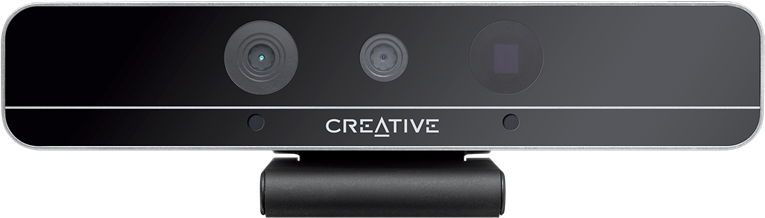
\includegraphics[width=.9\linewidth]{fig_intel_realsense}
\caption{The Intel RealSense sensor.}
\label{fig:intel_realsense}
\end{figure}

Another emerging technology, this time from Intel, is the RealSense (Figure \ref{fig:intel_realsense}). Intel RealSense, formerly known as Intel Perceptual Computing, is a platform for implementing gesture-based human-computer interaction (HCI) techniques. It consists of a series of consumer grade 3D cameras together with an easy to use machine perception library that simplifies supporting the cameras for third-party software developers \cite{bib_intel_real_sense}. An Intel RealSense camera contains the following four components: a conventional camera, an infrared laser projector, an infrared camera, and a microphone array. The infrared projector projects a grid onto the scene (in infrared light which is invisible to human eye) and the infrared camera records it to compute depth information. The microphone array allows localizing sound sources in space and performing background noise cancellation. Three camera models were announced, with distinct specifications and intended use, out of which the Intel RealSense 3D Camera (Front F200) is intended to be used for natural gesture-based interaction, face recognition, immersive video conferencing and collaboration, gaming, learning and 3D scanning.

\begin{figure}[htb]
\centering
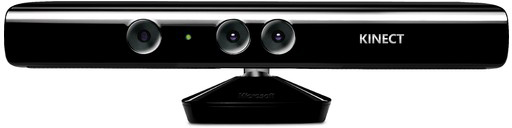
\includegraphics[width=.9\linewidth]{fig_microsoft_kinect_v1}
\caption{The Microsoft Kinect for Windows v1 sensor.}
\label{fig:microsoft_kinect_v1}
\end{figure}

Last, but not least, there is the Microsoft Kinect line-up of sensors (Figure \ref{fig:microsoft_kinect_v1}). Kinect (codenamed in development as ``Project Natal'') is a line of motion sensing input devices by Microsoft for Xbox 360 and Xbox One video game consoles and Windows PCs. Based around a webcam-style add-on peripheral, it enables users to control and interact with their console/computer without the need for a game controller, through natural user interface using gestures and spoken commands \cite{bib_microsoft_kinect_v1_sdk}. The first-generation Kinect was first introduced in November 2010 in an attempt to broaden Xbox 360's audience beyond its typical gamer base. A version for Windows was released on February 1, 2012. Kinect competes with several motion controllers on other home consoles, such as Wii Remote Plus for Wii and Wii U, PlayStation Move/PlayStation Eye for PlayStation 3, and PlayStation Camera for PlayStation 4. The Kinect sensor is a horizontal bar connected to a small base with a motorized pivot and is designed to be positioned lengthwise above or below the video display. The device features an RGB camera, depth sensor and multi-array microphone running proprietary software, which provide full-body 3D motion capture, facial recognition and voice recognition capabilities.

The depth sensor consists of an infrared laser projector combined with a monochrome CMOS sensor, which captures video data in 3D under any ambient light conditions. The sensing range of the depth sensor is adjustable, and Kinect software is capable of automatically calibrating the sensor based on gameplay and the player's physical environment, accommodating for the presence of furniture or other obstacles. According to information supplied to retailers, Kinect is capable of simultaneously tracking up to six people, including two active players for motion analysis with a feature extraction of 20 joints per player.

\subsection{Microsoft Kinect for Windows v2}

\begin{figure}[htb]
\centering
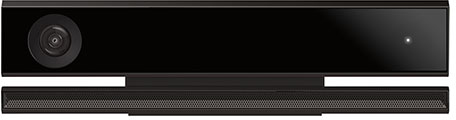
\includegraphics[width=.9\linewidth]{fig_microsoft_kinect_v2}
\caption{The Microsoft Kinect for Windows v2 sensor.}
\label{fig:microsoft_kinect_v2}
\end{figure}

The Microsoft Kinect for Windows v2 sensor (Figure \ref{fig:microsoft_kinect_v2}) is the successor of the v1, which was initially purposed for the Xbox 360 console but due to the rise in popularity of NUI applications was released afterwards for the desktop environments \cite{bib_microsoft_kinect_v2_sdk}. It brings significant improvements available for the next generation Kinect v2 camera. The biggest notable difference is the higher resolution capability of the Kinect v2 camera. Though the Kinect v1 device was a vast improvement over regular webcams, the Kinect v1 is restricted by its lower resolution output. From a pure technical specification standpoint, the community on MSDN has a product specification breakdown for Kinect v1 and Kinect v2 \cite{bib_msdn}.

The Kinect v2 face recognition, motion tracking, and resolution are much more precise than the Kinect v1. Kinect v2 uses ``time of flight'' technology to determine the features and motion of certain objects. It can be compared somewhat to sonar technology, except that this is a large improvement and more accurate. By using this, the Kinect v2 can see just as well in a completely dark room as in a well lit room. Although the first Kinect used similar technology, the Kinect v2 has greatly improved upon it. The Kinect v2 has 1080p resolution (HD).

Kinect v2 can process 2 GB of data per second; USB 3 provides almost 10 times faster broadband for the data transfer, 60\% wider field of vision, and can detect and track 20 joints from 6 people's bodies including thumbs. In comparison, the Kinect v1 could only track 20 joints from 2 people. On top of this, when using Kinect v2 we are capable of detecting facial expressions and weights on limbs, along with much more extremely valuable biometric data. The Kinect v1 device doesn't have the fidelity to individually track fingers and stretching and shrinking with hands and arms but the Kinect v2 has these capabilities. It's clear that this technology is certainly much more powerful and complex than the first generation of Kinect.

\subsection{Unity}

\begin{figure}[htb]
\centering
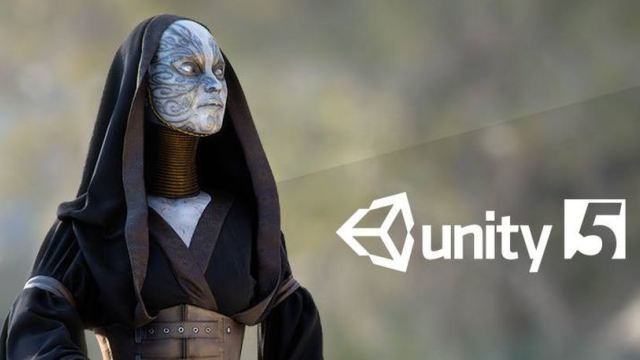
\includegraphics[width=.9\linewidth]{fig_unity_logo}
\caption{Unity 5 game engine.}
\label{fig:unity_logo}
\end{figure}

Unity (Figure \ref{fig:unity_logo}) is a cross-platform game engine developed by Unity Technologies and used to develop video games for PC, consoles, mobile devices and websites. With an emphasis on portability, the engine targets the following APIs: Direct3D on Windows and Xbox 360; OpenGL on Mac, Windows, and Linux; OpenGL ES on Android and iOS; and proprietary APIs on video game consoles. Unity provides support for bump mapping, reflection mapping, parallax mapping, screen space ambient occlusion (SSAO), dynamic shadows using shadow maps, render-to-texture and full-screen post-processing effects.

Unity is notable for its ability to target games to multiple platforms \cite{bib_unity}. Within a project, developers have control over delivery to mobile devices, web browsers, desktops, and consoles. Supported platforms include BlackBerry 10, Windows Phone 8, Windows, OS X, Linux (mainly Ubuntu), Android, iOS, Unity Web Player (including Facebook), Adobe Flash, PlayStation 3, PlayStation 4, PlayStation Vita, Xbox 360, Xbox One, Wii U, New 3DS and Wii. This high portability factor together with its shallow learning curve made it our main choice as a rendering framework.

\begin{figure}[htb]
\centering
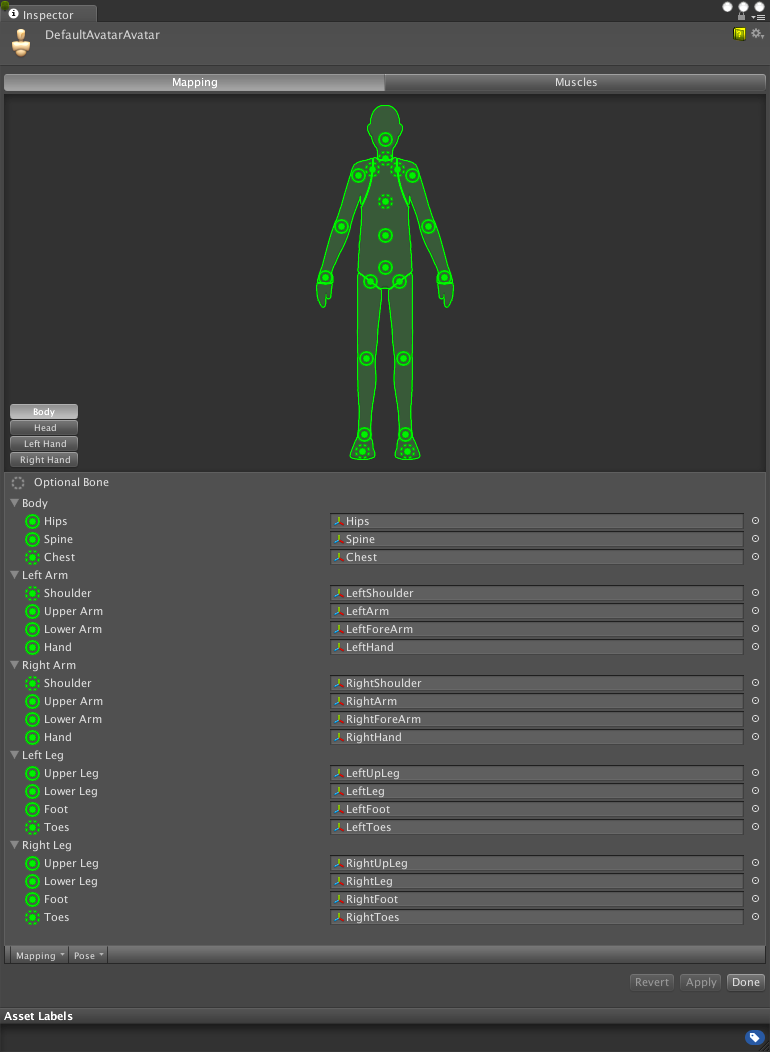
\includegraphics[width=.9\linewidth]{fig_mecanim_hierarchy}
\caption{Unity 5 Mecanim bone hierarchy.}
\label{fig:mecanim_hierarchy}
\end{figure}

Unity has a rich and sophisticated animation system called Mecanim - Figure \ref{fig:mecanim_hierarchy}. Mecanim provides:

\begin{itemize}
\item Easy workflow and setup of animations for all elements of Unity including objects, characters, and properties;
\item Support for imported animation clips and animations created within Unity;
\item Humanoid animation retargeting - the ability to apply animations from one character model onto another;
\item Simplified workflow for aligning animation clips;
\item Convenient preview of animation clips, transitions and interactions between them; this allows animators to work more independently of programmers, prototype and preview their animations before gameplay code is hooked in;
\item Management of complex interactions between animations with a visual programming tool;
\item Animating different body parts with different logic;
\item Layering and masking features;
\end{itemize}

Unity's animation system is based on the concept of animation clips, which contain information about how certain objects should change their position, rotation, or other properties over time. Each clip can be thought of as a single linear recording. Animation clips from external sources are created by artists or animators with 3rd party tools such as Max or Maya, or come from motion capture studios or other sources. Animation clips are then organised into a structured flowchart-like system called an animator controller. The animator controller acts as a ``state machine'' which keeps track of which clip should currently be playing, and when the animations should change or blend together.

A very simple animator controller might only contain one or two clips, for example to control a power-up spinning and bouncing, or to animate a door opening and closing at the correct time. A more advanced animator controller might contain dozens of humanoid animations for all the main character's actions, and might blend between multiple clips at the same time to provide a fluid motion as the player moves around the scene. Unity's animation system also has numerous special features for handling humanoid characters which give you the ability to retarget humanoid animation from any source (motion capture, the asset store, or some other third-party animation library) to your own character model, as well as adjusting muscle definitions. These special features are enabled by Unity's avatar system, where humanoid characters are mapped to a common internal format. Each of these pieces - the animation clips, the animator controller, and the avatar, are brought together on a game object via the animator component. This component has a reference to an animator controller, and (if required) the avatar for this model. The animator controller, in turn, contains the references to the animation clips it uses.

\subsection{Mixamo}

\begin{figure}[htb]
\centering
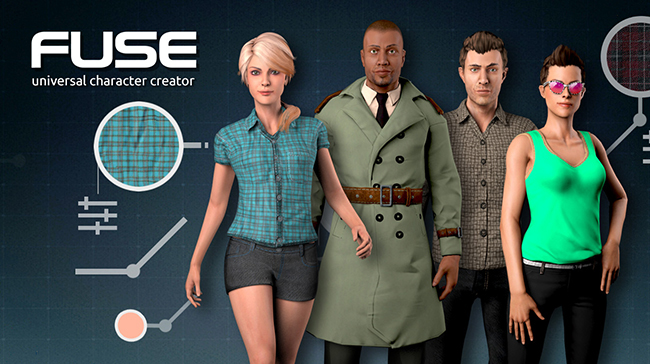
\includegraphics[width=.9\linewidth]{fig_mixamo_logo}
\caption{Mixamo animation services.}
\label{fig:mixamo_logo}
\end{figure}

Mixamo (Figure \ref{fig:mixamo_logo}) is a 3D computer graphics technology company, based in San Francisco, which develops and sells web-based services for 3D character animation. Mixamo's technologies use machine learning methods to automate the steps of the character animation process, including 3D modelling to rigging and 3D animation. In March 2014, Mixamo officially launched Fuse Character Creator at Game Developers Conference (GDC). It allows users to create a 3D character by assembling customizable body parts, clothing and textures together \cite{bib_mixamo}. Those characters can then be exported into other 3D model software packages or game engine.

Mixamo also provides an online, automatic model rigging service known as the Auto-Rigger, which was the industry's first online rigging service. The AutoRigger applies machine learning to understand where the limbs of a 3D model are and to insert a ``skeleton'', or rig, into the 3D model as well as calculating the skinning weights (the service can take up to 2 minutes). Mixamo's online services include an animation store featuring downloadable 3D models and animation sequences. The animations were created at Mixamo using motion capture and cleaned up by key frame animators. All its animations work with characters created in Fuse and/or rigged with Mixamo's AutoRigger.

\clearpage

\section{Architecture overview}

In order to reach the present architecture, the framework has undergone a process of iterative, stepwise refinement, starting from the initial specification - that of a solution that enables motion capture from the Kinect sensor and ending in a project with the functionalities discussed in the previous sections. To illustrate this, we have chosen to describe the decisions we took during the development phase.

First we analysed the problem statement which implies two components: a hardware sensor and an animation system alongside a game engine. For the former, we opted for Microsoft's Kinect v2 sensor since it best suited our range of application, namely actors/individuals recording animations at home and not a professional studio. It provides the required tracking precision for a person's movements and can optionally track multiple bodies within the confines of the same scene. We aim to exploit this capability in future releases of Reflecta for example to animate an entire crowd of 3D characters simultaneously.

As for the game engine, Unity's latest release - Unity 5 clearly is ahead of the competition in terms of the learning curve required to build a functional game in as short amount of time as possible. Plus, it can target multiple platforms and allows us to focus more on the logic of the application, abstracting away the complex inner workings of a game engine. Unity ships with an integrated animation system called Mecanim, which we have used extensively.

After this phase, we took the decision to divide Reflecta into two loosely coupled applications, which will be referenced in the following sections as ``server'' and ``client''. This design allows us to swap the two components with other, custom made implementations, whilst still retaining the overall behaviour of the system. The general flow of Reflecta is as follows:

\begin{itemize}
\item The server captures a motion frame as it arrives from the sensor;
\item The server sends the raw frame data to the client;
\item The client interprets the raw data and animates a 3D avatar;
\item The client captures the rendered output;
\item The client sends the rendered output back to the server;
\item The server displays the received image on screen;
\end{itemize}

Of specific interest to the reader is the fact that the server only relays the raw data from the sensor and does not process it by any means. This contributes to the design of Reflecta by enforcing a loose coupling between the server and client. The client is the one responsible for interpreting the raw data into a format more suitable for its internal animation system. Furthermore, the server is expecting back an rendered image, with no specification from whence it came from. Thus clients can be swapped for implementations made with other game engines, as long as this protocol holds true.

Since the server and client are two separate applications, the question arises about what type of communication channel we should utilize. TCP or UDP favour a distributed design, but in most cases Reflecta would run on the same machine. Then again, sending back the rendered output from client to server requires significant bandwidth. The client-server frames are the raw bytes from Unity's renderer output (note the order of the server and client entities). In our particular case we render at a resolution of 720p at 25 FPS, which amounts to roughly 88 MBps. We have found that the best balance is provided by using named pipes.

The next decision we faced was upon the communication protocol. We envisioned Reflecta from the start as being a multi purpose NUI solution, not just an animation tool, and we designed it to integrate with other frameworks such as Microsoft's speech synthesis and recognition library. As a consequence all server-client (note again the order) communication is done in the form of commands. Commands need to be serialized to persist between client and server. Multiple serialization protocols exist: XML, JSON, .NET's own serialization and ProtoBuf (Google's Protocol Buffers) to name a few. XML and JSON have the advantage of being human-readable, but the size of the serialized output can be considerable, due to them being textual formats. Because we already take up a lot of memory for the client-server channel, this rules out these two options. 

As opposed to this, .NET's serialization mechanism produces a binary format of acceptable size, but can only be deserialized within the same version of the serialization library that yielded the output \cite{bib_msdn}. To be noted that, in order to develop an application with the Kinect for Windows v2 sensor, one must target at least the .NET Framework 4.5.2. In contrast, Unity 5 uses a subset version of the .NET Framework 3.5 and consequently, the native .NET serialization is also ruled out. The remaining candidate, protobuf or Google's Protocol Buffers best fits our scenario. It is both a compact binary serialization and provides libraries supporting .NET Framework 2.0 up to the latest .NET Framework \cite{bib_google_protocol_buffers}.

In our particular case, the server is a Windows Forms application responsible for interfacing with the Kinect hardware and motion capture data acquisition, whilst the client interprets the data and renders the output which in turn is sent back to the server which displays it in a custom designed per pixel alpha form. The server-client packages are protocol buffer-serialized commands. The client-server frames are the raw bytes of the rendered output. For a graphical representation of this process please refer to Figure \ref{fig:reflecta_architecture}.

\begin{figure}[htb]
\centering
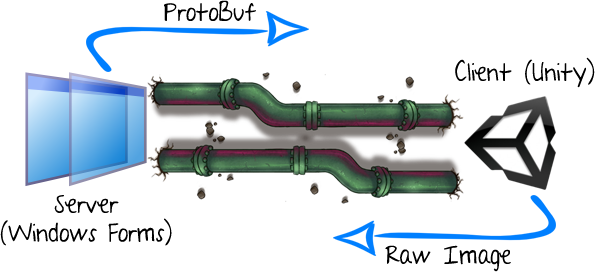
\includegraphics[width=.9\linewidth]{fig_reflecta_architecture}
\caption{Reflecta architecture diagram.}
\label{fig:reflecta_architecture}
\end{figure}

\subsection{Advantages and drawbacks}

The authors would like to reiterate their opinions on the aforementioned architecture:

Advantages:

\begin{itemize}
\item Decoupling application into server and client yields a clear separation of responsibility;
\item Overall code becomes cleaner and more concise;
\item It is possible to plug in other client implementations as long as the pipeline stays the same;
\item Aids development in the wider field of NUI applications by providing support for speech synthesis/recognition;
\item Mocap data is stored as a raw protobuf which means it is readily available to third party animation systems;
\end{itemize}

Drawbacks:

\begin{itemize}
\item Have to provide an extra layer of abstraction situated above the Kinect and Unity animation systems;
\item Need to define the Kinect body skeleton, the Mecanim avatar body joints and map between them; this is not always possible as we shall see later on;
\item Need to define the Kinect facial expression system, which is based on the Candide-3 model, the Mixamo rig facial blends and map between them (again, these do not map on to one);
\item Must implement our own mathematical computation library since we can not include dependencies to Unity's math structures and operations;
\end{itemize}

\subsection{Our own math library}

The core of Reflecta is built upon the structures that are most commonly used in 3D graphics: vectors and quaternions. Vectors usually come in 2, 3 and 4 dimensional flavours, but only the 3D vector is needed in most cases. It can be used to represent 3D positions or to store rotations as Euler angles around the X, Y and Z axes respectively. It is common knowledge that the Euler angles representation suffers from the gimbal lock phenomenon, where rotations tend to flip at boundary values for the given angles. The quaternion can be compared to a 4D vector, in the sense that it stores 4 components, X, Y, Z and W. But the similarities end here; the extra dimension means that, for a given Euler angle representation, we have an infinite number of quaternions representing the same rotation. The X, Y and Z components of a quaternion store the axis of rotation, and the W component - the amount or angle of rotation around that axis \cite{bib_quaternions}.

\begin{lstlisting}[basicstyle=\tiny]
[ProtoContract]
public struct Vector3
{
    [ProtoMember(1)] public float X;
    [ProtoMember(2)] public float Y;
    [ProtoMember(3)] public float Z;
}
\end{lstlisting}

\begin{lstlisting}[basicstyle=\tiny]
[ProtoContract]
public struct Quaternion
{
    [ProtoMember(1)] public float X;
    [ProtoMember(2)] public float Y;
    [ProtoMember(3)] public float Z;
    [ProtoMember(4)] public float W;
}
\end{lstlisting}

Our math library started from an open source port of the Microsoft XNA Framework called MonoGame \cite{bib_mono_game}, but we have extended the framework to support more complex operations on the types we defined earlier such as advanced slerp (spherical interpolation for quaternions), quaternion neighbourhood checking and conversion to and from Euler angles (with proper handling of limit cases) - Figure \ref{fig:reflecta_math}.

\begin{figure}[htb]
\centering
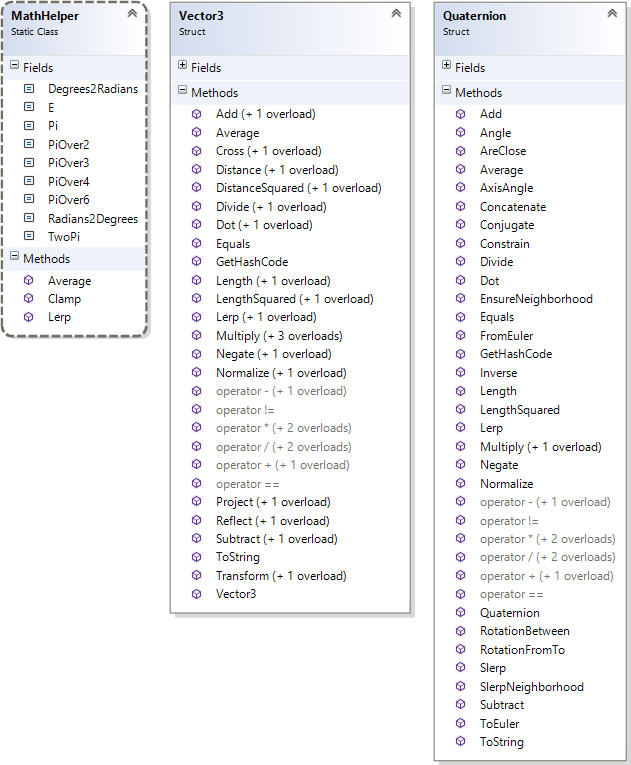
\includegraphics[width=.9\linewidth]{fig_reflecta_math}
\caption{Overview of the math operations exposed by Reflecta.}
\label{fig:reflecta_math}
\end{figure}

Remark the presence of an ``average'' method for computing the average value of an array of a basic type in all entities as this will be of significant importance in the future sections, especially in the noise reduction discussion.

\subsection{Basic and compound entities}

The types described above constitute the basic types of Reflecta. On top of these objects, we build progressively more complex entities (Figure \ref{fig:reflecta_compound_entities}) by means of the ``has-a'' relationship, eventually reaching a mocap data structure which holds our representation of the recorded raw motion frames coming from the Kinect sensor.

\begin{figure}[htb]
\centering
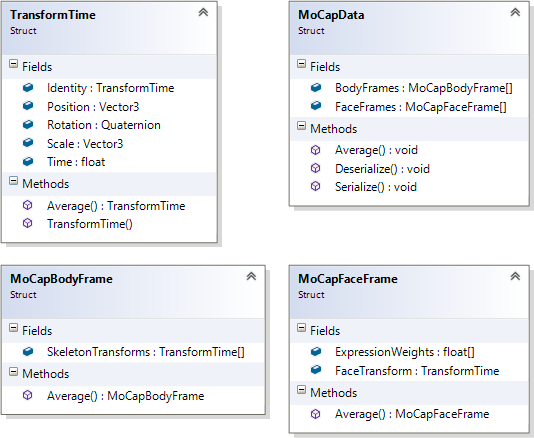
\includegraphics[width=.9\linewidth]{fig_reflecta_compound_entities}
\caption{Overview of the compound entities which make up Reflecta.}
\label{fig:reflecta_compound_entities}
\end{figure}

TransformTime holds a position (Vector3), rotation (Quaternion), scale (Vector3) similar to the transform employed by Unity, and additionally, a float value which specifies the time of the current keyframe. To be more specific, TransformTime stores the description of a single body bone in a discrete time frame.

The MoCapBodyFrame represents a snapshot of all the body joints at a given moment of time, and internally stores an array of transforms indexed by the bone indices of the skeleton. In a similar fashion, the MoCapFaceFrame holds an array of expression weights, indexed by the indices of the available facial morphs, plus the head transform of the currently tracked subject.

Finally, the MoCapData is a collection of all body and face frames that have arrived since the recording started, effectively making it our internal representation of an animation. It offers support for serialization/deserialization by use of protocol buffers. We would like to emphasize that this format is very compact, with recordings in the order of minutes taking up less than 1 MB.

The relationships between the various core entities are further detailed in Figures \ref{fig:reflecta_entity_relationships_basic}, \ref{fig:reflecta_entity_relationships_bones}, \ref{fig:reflecta_entity_relationships_expressions}, \ref{fig:reflecta_entity_relationships_desp} and \ref{fig:reflecta_entity_relationships_pipeline}.

\begin{figure}[htb]
\centering
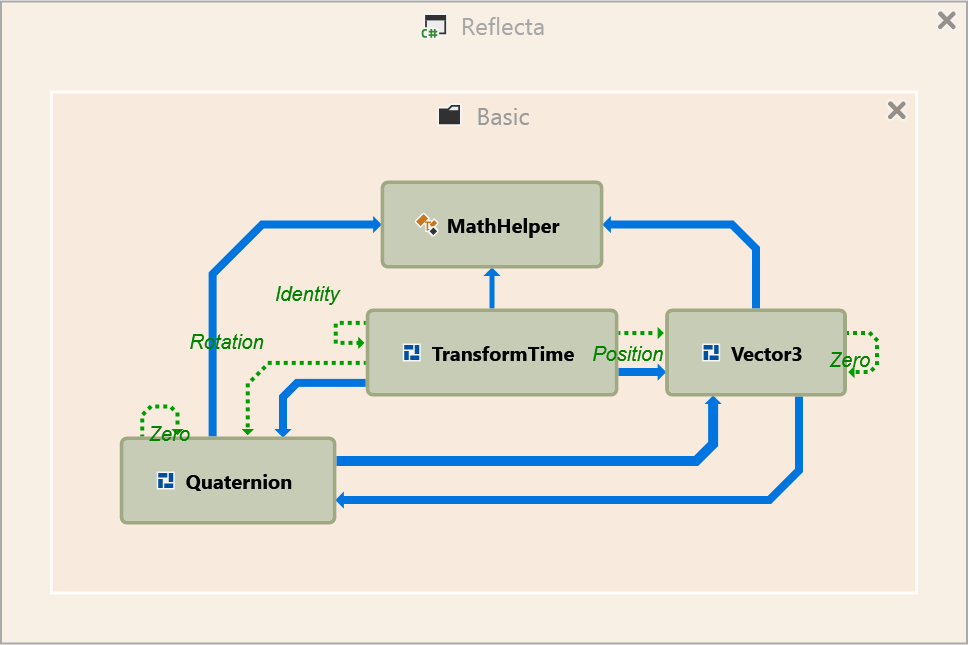
\includegraphics[width=.6\linewidth]{fig_reflecta_entity_relationships_basic}
\caption{Basic entities.}
\label{fig:reflecta_entity_relationships_basic}
\end{figure}

\begin{sidewaysfigure}[htb]
\vspace{100mm}
\centering
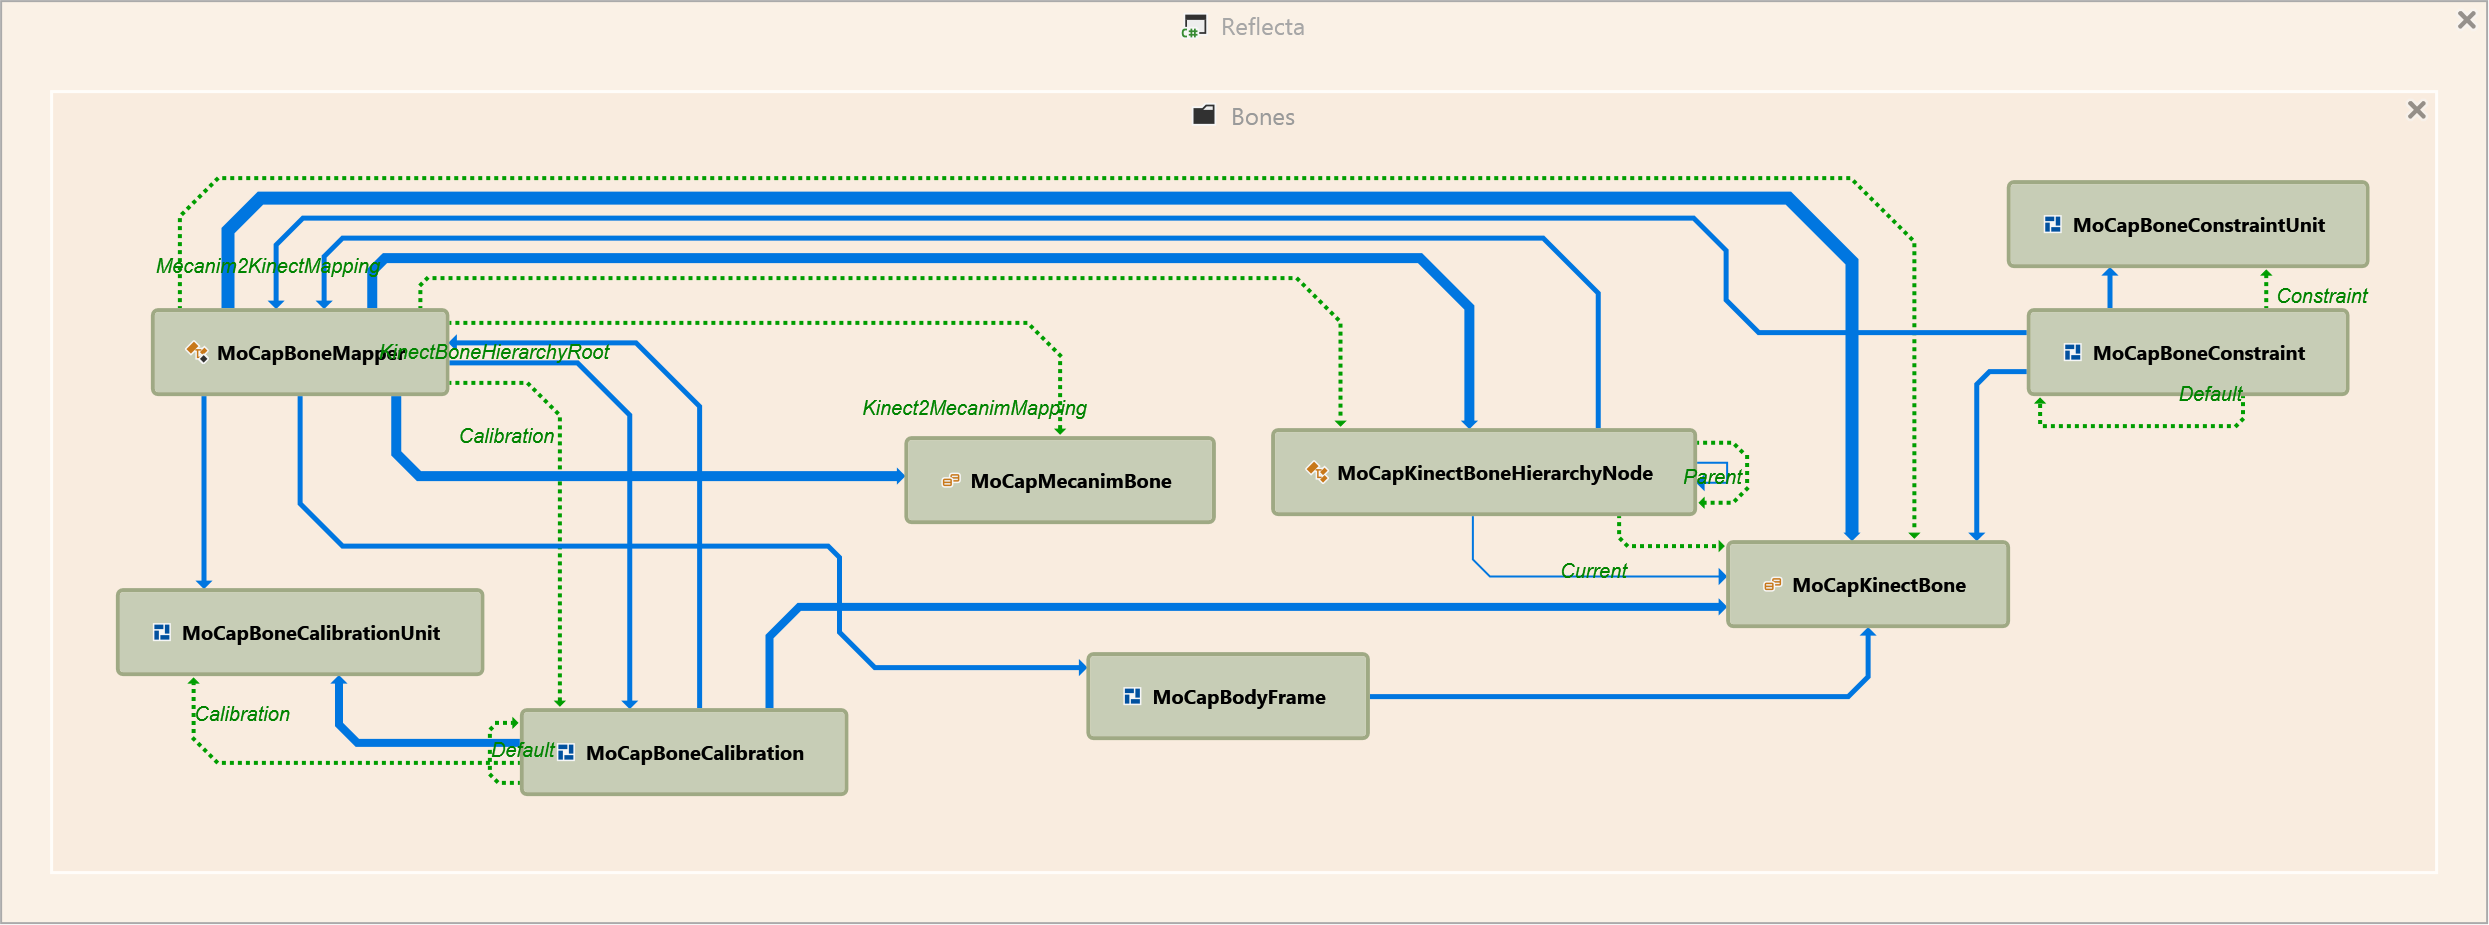
\includegraphics[width=1\linewidth]{fig_reflecta_entity_relationships_bones}
\caption{Skeleton bone-related entities.}
\label{fig:reflecta_entity_relationships_bones}
\end{sidewaysfigure}

\begin{sidewaysfigure}[htb]
\vspace{100mm}
\centering
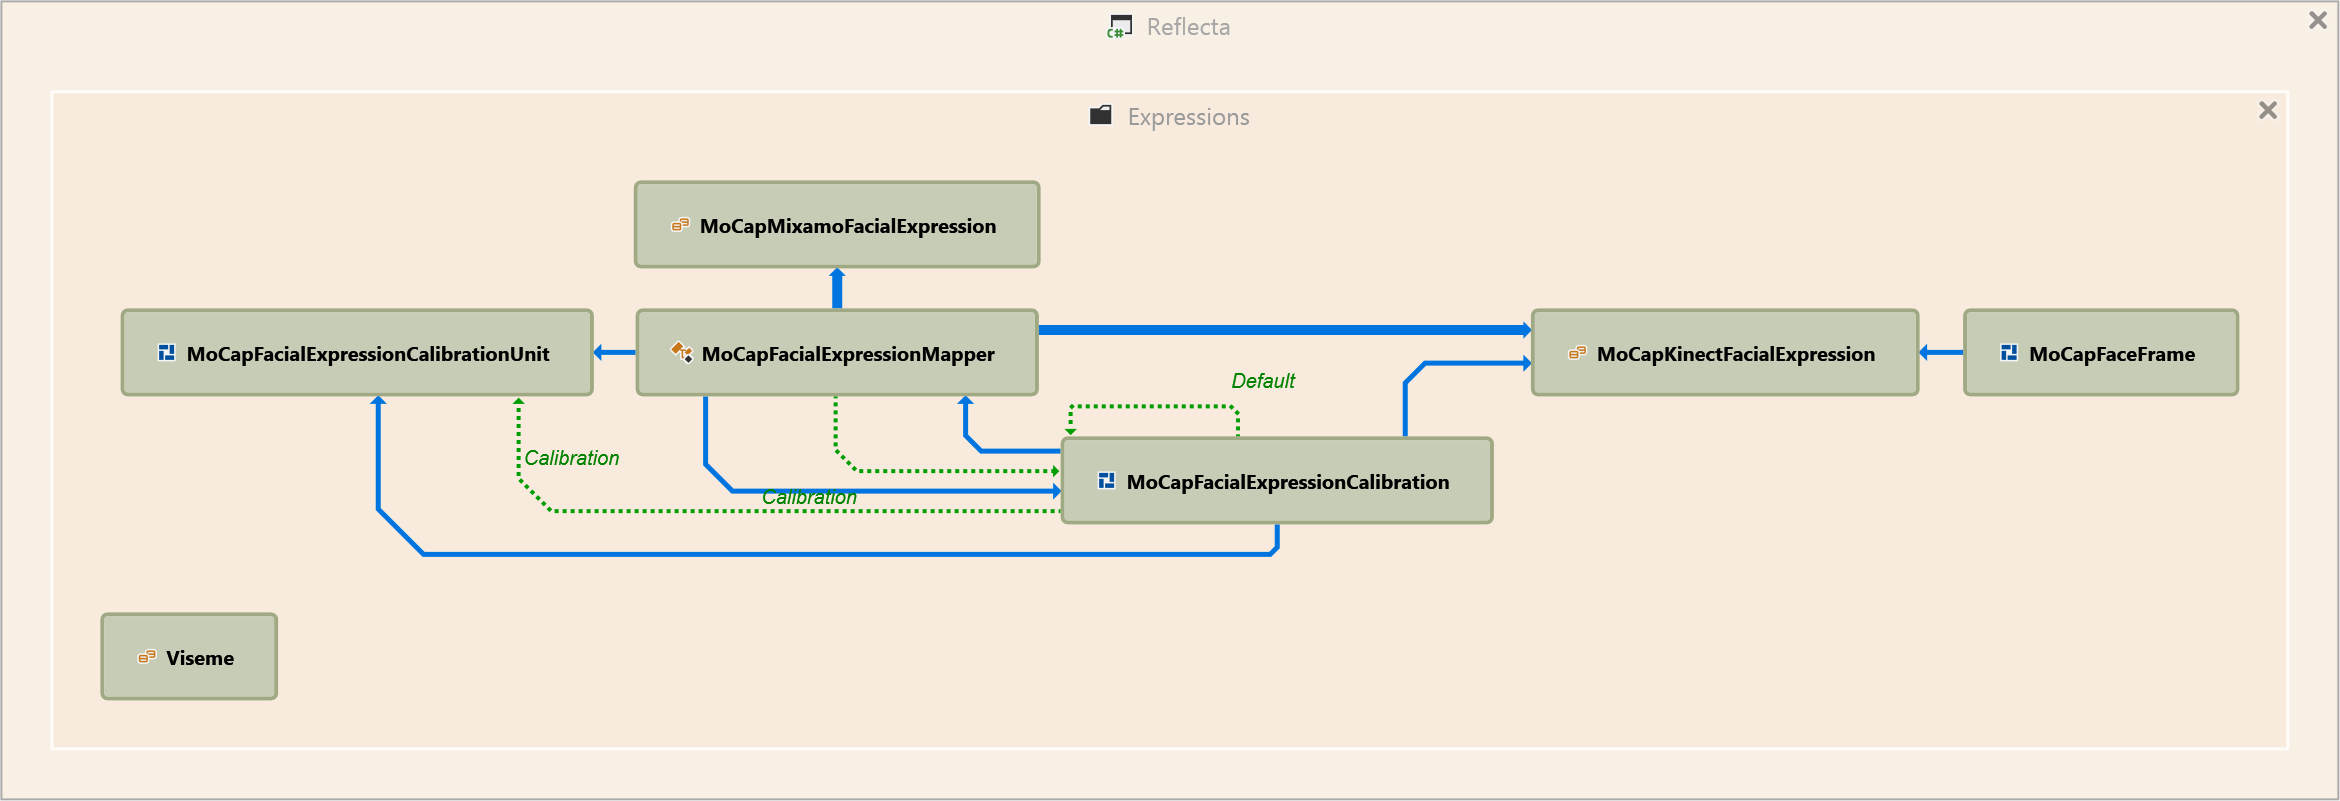
\includegraphics[width=1\linewidth]{fig_reflecta_entity_relationships_expressions}
\caption{Facial morph-related entities.}
\label{fig:reflecta_entity_relationships_expressions}
\end{sidewaysfigure}

\begin{figure}[htb]
\centering
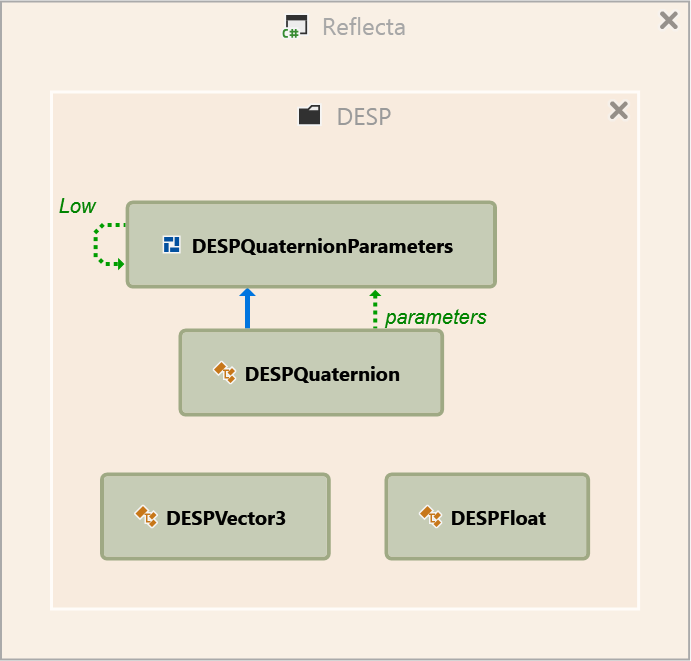
\includegraphics[width=.6\linewidth]{fig_reflecta_entity_relationships_desp}
\caption{DESP-related entities.}
\label{fig:reflecta_entity_relationships_desp}
\end{figure}

\begin{figure}[htb]
\centering
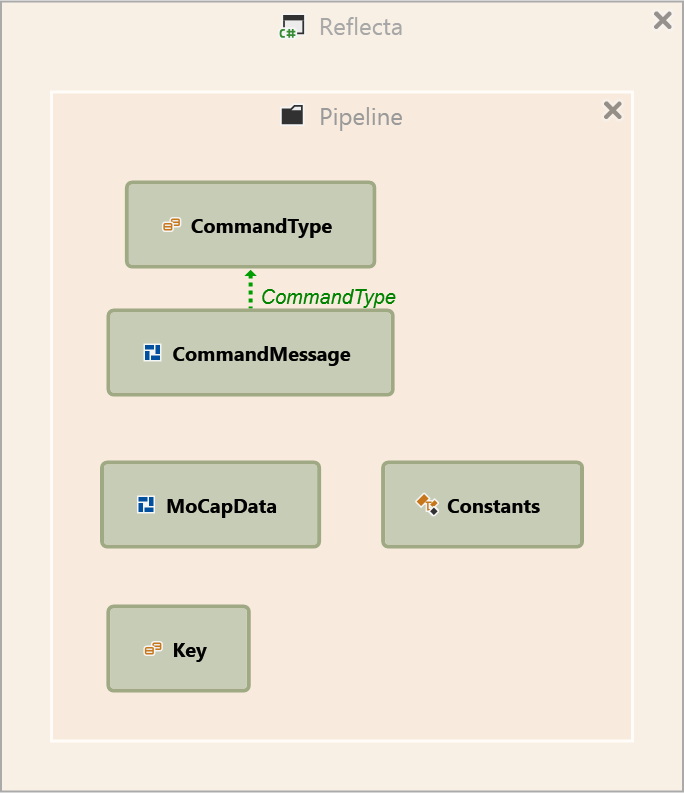
\includegraphics[width=.6\linewidth]{fig_reflecta_entity_relationships_pipeline}
\caption{General pipeline-related entities.}
\label{fig:reflecta_entity_relationships_pipeline}
\end{figure}

\clearpage

\section{Handling body data}
Body joint data arrives from the Kinect in the form of quaternions representing bone orientations in the Kinect world space, in absolute hierarchical values \cite{bib_microsoft_kinect_v2_sdk}. Unity animations, on the other hand operate on local rotations \cite{bib_unity}. The formula for computing the local rotation from an absolute global rotation \cite{bib_quaternions} is given in \eqref{eq:quaternion_global_to_local}, where ``parent'' denotes the parent of the current bone in the bone hierarchy - Figure \ref{fig:kinect_skeleton}.

\begin{figure}[htb]
\centering
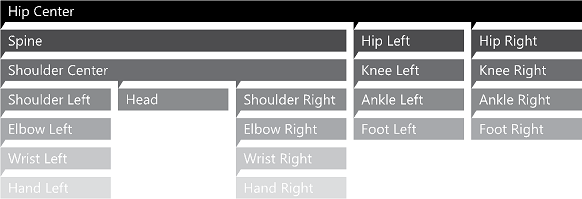
\includegraphics[width=.9\linewidth]{fig_kinect_skeleton}
\caption{Kinect skeleton.}
\label{fig:kinect_skeleton}
\end{figure}

\begin{equation} \label{eq:quaternion_global_to_local}
Q_{current\_local} = Q_{parent\_absolute}^{-1} * Q_{current\_absolute}
\end{equation}

The Kinect bone orientations are not readily usable in Unity, as we have found out through trial and error. Thus, compensation factors need to be applied when extrapolating the local rotation from the absolute rotation. This responsibility is delegated in our implementation to the MoCapBoneCalibration class, which effectively stores quaternion compensations to be multiplied with the result from \eqref{eq:quaternion_global_to_local} in order to get physically accurate results.

As we have pointed out before, the Kinect and Mecanim skeletons do not correspond one to one. Below (Figure \ref{fig:reflecta_bone_enumerations}) we give the exact bone enumerations, at the moment this paper was written (note that this is probably subject to change). There are 25 Kinect bones as opposed to 54 Mecanim bones.

\begin{figure}[htb]
\centering
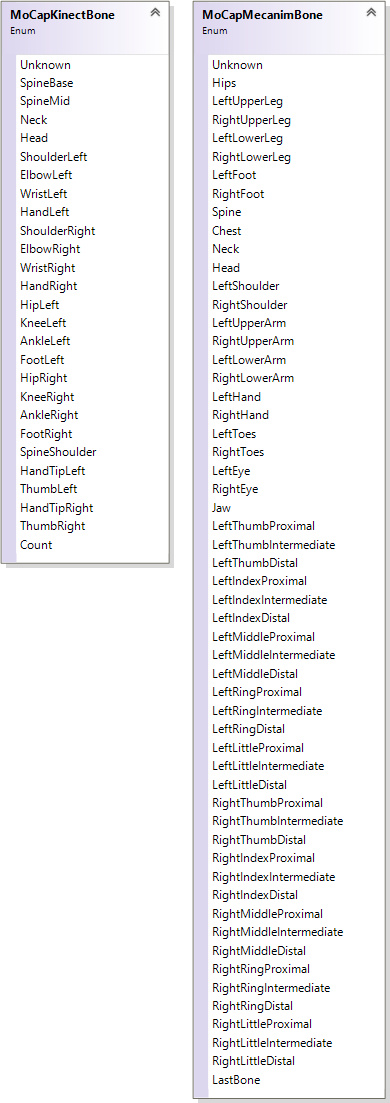
\includegraphics[width=.575\linewidth]{fig_reflecta_bone_enumerations}
\caption{Kinect bones vs. Mecanim bones.}
\label{fig:reflecta_bone_enumerations}
\end{figure}

\subsection{Custom bone mapping}

We have provided functions to map from one bone hierarchy to another. Our version of the direct mapping between Kinect and Mecanim is the following:

\begin{lstlisting}[basicstyle=\tiny]
Map[Kinect.SpineBase] = Mecanim.Hips;
Map[Kinect.SpineMid] = Mecanim.Spine;
Map[Kinect.SpineShoulder] = Mecanim.Chest;
Map[Kinect.Neck] = Mecanim.Neck;
Map[Kinect.Head] = Mecanim.Head;

Map[Kinect.ShoulderLeft] = Mecanim.RightShoulder;
Map[Kinect.ElbowLeft] = Mecanim.RightUpperArm;
Map[Kinect.WristLeft] = Mecanim.RightLowerArm;
Map[Kinect.HandLeft] = Mecanim.RightHand;
Map[Kinect.ThumbLeft] = Mecanim.RightThumbDistal;
Map[Kinect.HandTipLeft] = Mecanim.RightMiddleDistal;

Map[Kinect.ShoulderRight] = Mecanim.LeftShoulder;
Map[Kinect.ElbowRight] = Mecanim.LeftUpperArm;
Map[Kinect.WristRight] = Mecanim.LeftLowerArm;
Map[Kinect.HandRight] = Mecanim.LeftHand;
Map[Kinect.ThumbRight] = Mecanim.LeftThumbDistal;
Map[Kinect.HandTipRight] = Mecanim.LeftMiddleDistal;

Map[Kinect.HipLeft] = Mecanim.Unknown;
Map[Kinect.KneeLeft] = Mecanim.RightUpperLeg;
Map[Kinect.AnkleLeft] = Mecanim.RightLowerLeg;
Map[Kinect.FootLeft] = Mecanim.RightFoot;

Map[Kinect.HipRight] = Mecanim.Unknown;
Map[Kinect.KneeRight] = Mecanim.LeftUpperLeg;
Map[Kinect.AnkleRight] = Mecanim.LeftLowerLeg;
Map[Kinect.FootRight] = Mecanim.LeftFoot;
\end{lstlisting}

Please remark that we have swapped left joints for right joints and vice-versa when mapping between the two systems. This is because we want the rendered 3D model to be a mirrored image of the actual person standing in front of the Kinect sensor.

\clearpage

\section{Handling facial expression data}

The Kinect input follows the Candide-3 model \cite{bib_candide_3}, whilst on the other hand Mixamo uses its own proprietary system for facial expression morphs (Figure \ref{fig:reflecta_face_enumerations}). Furthermore, the SDK documentation for the Kinect v2 sensor states that expression weights are in the range [-1, 1] \cite{bib_microsoft_kinect_v2_sdk}. In practice, we have found that this differs from action unit to action unit and face recognition quality is also subject to lighting conditions. To alleviate this issue, we have implemented a MoCapFacialExpressionMapper helper class responsible with computing the actual mapping between the two animation systems. An important remark to be made here is that one expression from the Kinect can have multiple mappings (usually at most two) in the Mixamo system. The Kinect provides a total of 17 facial expressions, where as Mixamo has 50 available facial blend shapes.

\begin{figure}[htb]
\centering
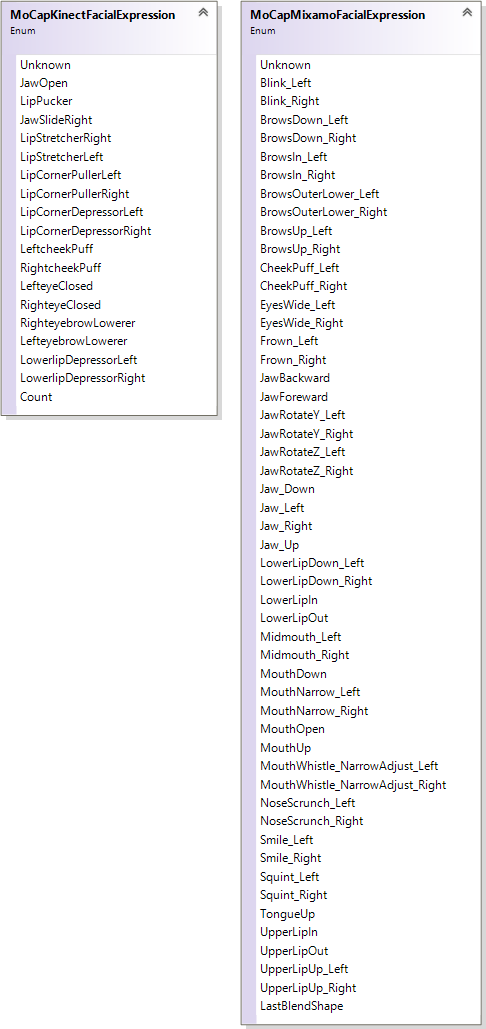
\includegraphics[width=.6\linewidth]{fig_reflecta_face_enumerations}
\caption{Kinect facial expressions vs. Mixamo blend shapes.}
\label{fig:reflecta_face_enumerations}
\end{figure}

\subsection{Custom facial expression mapping}

Again, the two systems need an actual mapping:

\begin{lstlisting}[basicstyle=\tiny]
JawOpen => Jaw_Down;
LipPucker => NULL;
JawSlideRight => Jaw_Right/Jaw_Left;
LipStretcherRight => NULL;
LipStretcherLeft => NULL;
LipCornerPullerLeft => Smile_Left;
LipCornerPullerRight => Smile_Right;
LipCornerDepressorLeft => Frown_Left;
LipCornerDepressorRight => Frown_Right;
LeftcheekPuff => CheekPuff_Left;
RightcheekPuff => CheekPuff_Right;
LefteyeClosed => Blink_Left;
RighteyeClosed => Blink_Right;
RighteyebrowLowerer => BrowsDown_Right/BrowsUp_Right;
LefteyebrowLowerer => BrowsDown_Left/BrowsUp_Left;
LowerlipDepressorLeft => LowerLipDown_Left;
LowerlipDepressorRight => LowerLipDown_Right;
\end{lstlisting}

\clearpage

\section{Handling input noise}

Noise is inherent to all sensor hardware, and the Kinect is by no means an exception. On the contrary, we have found it very susceptible to environmental lighting conditions. In the current literature there exist a multitude of solutions that tackle the noise problem ranging from a simple average of the frames over a certain time period to Kalman filter based predictors \cite{bib_kalman}. We have opted for a combined approach which we consider provides a good balance between computational cost and noise reduction efficiency.

\subsection{Simple average}

The simplest version of a noise reduction algorithm employs a queue of mocap data frames over a given time interval and, upon request, evaluates the average of the frame values and outputs a result. Depending on the queue size, the behaviour of the output can vary: a smaller queue size leads to a more responsive avatar, with increased joint jitter (noise in rotation values); a larger queue size has the effect of a ``laggy'' animation, but with smoother movement. After a number of experiments, in order to strike a balance in our implementation, we have set the queue size to a value of 8. A further improvement would be to have a dynamic queue size, based on an analysis of the environmental conditions.

In the previous sections we pointed out that all our entities have support for this averaging scheme.

\subsection{DESP}

DESP or double exponential smoothing prediction \cite{bib_desp} is a relatively cheap computational alternative to Kalman filter based prediction while simultaneously achieving similar noise reduction quality. It is designed for continuous streams of input and has the added bonus of being capable to ``predict'' a number of frames into the future based on the trend of the input. The DESP keeps track of two statistics regarding the evolution of the input \eqref{eq:desp_statistics}.

\begin{equation} \label{eq:desp_statistics}
\begin{split}
S_{p_{t}} = \alpha * p_{t} + (1 - \alpha) * S_{p_{t - 1}}
\\
S_{p_{t}}^{'} = \alpha * S_{p_{t}} + (1 - \alpha) * S_{p_{t - 1}}^{'}
\end{split}
\end{equation}

Note the alpha parameter, which is a property of the predictor as a whole and affects the ``weight'' of the previous frames with respect to the current frame in evaluating the prediction. Alpha is expected to be in the range [0, 1], with values closer to 0 leading to a very aggressive smoothing, with very high input lag and values closer to one making the avatar more responsive, at the cost of little noise reduction. In our particular case we typically use a value between 0.25 and 0.5.

We have designed predictors for the Reflecta basic types: float, Vector3 and Quaternion with the server component managing instances of these predictors for each joint/facial expression which are continuously fed data from the Kinect sensor. With respect to their implementation, the first two predictors are very similar, the Vector3 version being a per-component application of its float counterpart. Below one can find the full listing of the float DESP.

\begin{lstlisting}[basicstyle=\tiny]
public sealed class DESPFloat
{
    public float alpha=0.5f;
    private float crt_stat_1;
    private float crt_stat_2;
    private float prev_stat_1;
    private float prev_stat_2;

    public void Update(float value)
    {
        crt_stat_1=alpha*value+(1-alpha)*prev_stat_1;
        crt_stat_2=alpha*crt_stat_1+(1-alpha)*prev_stat_2;

        prev_stat_1=crt_stat_1;
        prev_stat_2=crt_stat_2;
    }

    public float Predict(int tau)
    {
        var factor=alpha/(1-alpha)*tau;
        return (2+factor)*crt_stat_1-(1+factor)*crt_stat_2;
    }

    public float Predict(float tau)
    {
        var floor=(int)Math.Floor(tau);
        var ceiling=(int)Math.Ceiling(tau);

        var lo=Predict(floor);
        var hi=Predict(ceiling);

        var rho=tau-floor;

        return MathHelper.Lerp(lo, hi, rho);
    }
}
\end{lstlisting}

Here, the overloaded prediction function takes as parameter the number of frames we wish to estimate into the future. In the first case, the parameter is of integral type, but the second can accept a floating point value. Here the estimation is computed by calculating the floor and ceiling of the parameter (which yields an integer) and linearly interpolating between the two.

Handling quaternions is a bit more complicated. The original authors of the DESP paper \cite{bib_desp} suggest applying computation in a similar fashion to the vector DESP, with a slerp operation for interpolation, instead of a simple lerp. In practice, we have found that this introduces discontinuities for joint movements in certain ranges. A solution would be to constrain the bone rotation to certain human observer ranges. However this forces us to convert quaternions to Euler angles, which beats the purpose of using quaternions to store rotations. Our approach uses a modified version of the quaternion DESP, which exposes additional parameters such as correction, jitter radius, maximum deviation radius, prediction and smoothing.

\begin{lstlisting}[basicstyle=\tiny]
public Quaternion Predict(Quaternion value)
{
    var filteredOrientation = Quaternion.Zero;
    var trend = Quaternion.Zero;

    var diffJitter = Quaternion.RotationBetween(value, 
        prevFilteredOrientation);
    var diffJitterValue = Math.Abs(Quaternion.Angle(diffJitter));
    if (diffJitterValue <= parameters.JitterRadius)
        filteredOrientation = Quaternion.SlerpNeighborhood(
            prevFilteredOrientation, value,
            diffJitterValue/parameters.JitterRadius);
    else
        filteredOrientation = value;
    filteredOrientation = Quaternion.SlerpNeighborhood(
        filteredOrientation,
        prevFilteredOrientation*prevTrend,
        parameters.Smoothing);
    diffJitter = Quaternion.RotationBetween(filteredOrientation, 
        prevFilteredOrientation);

    trend = Quaternion.SlerpNeighborhood(prevTrend, diffJitter,
        parameters.Correction);

    var predictedOrientation = filteredOrientation*
                               Quaternion.SlerpNeighborhood(
                                   Quaternion.Identity, trend,
                                   parameters.Prediction);

    var diff = Quaternion.RotationBetween(predictedOrientation, 
        filteredOrientation);
    var diffValue = Math.Abs(Quaternion.Angle(diff));
    if (diffValue > parameters.MaxDeviationRadius)
        predictedOrientation = Quaternion.SlerpNeighborhood(
            filteredOrientation, predictedOrientation,
            parameters.MaxDeviationRadius/diffValue);

    predictedOrientation = Quaternion.Normalize(predictedOrientation);
    filteredOrientation = Quaternion.Normalize(filteredOrientation);
    trend = Quaternion.Normalize(trend);

    prevFilteredOrientation = filteredOrientation;
    prevTrend = trend;

    return predictedOrientation;
}
\end{lstlisting}

\subsection{A combined approach}

In most situations it is useful to approach a problem by a combination of various techniques, which one considers useful and experiment with them. The current version of Reflecta employs DESP prediction for joint orientations (quaternion DESP) and facial expression weights (float DESP). These are stored server-side such that the final mocap data structure benefits from integrated noise smoothing. The frame queue mechanism is employed by the Unity client which averages the incoming frames from the server.

There is one extra aspect we wish to discuss and it refers to the facial blend weights. The Kinect documentation states that the values are in the range [0, 1] or [-1, 1] depending on expression type. In actual, real world usage, these ranges vary per-expression:

\begin{lstlisting}[basicstyle=\tiny]
    <!--JawOpen-->
      <WeightMin>0.00</WeightMin>
      <WeightMax>0.40</WeightMax>
    <!--LipPucker-->
      <WeightMin>0.00</WeightMin>
      <WeightMax>0.80</WeightMax>
    <!--JawSlideRight-->
      <WeightMin>-0.25</WeightMin>
      <WeightMax>0.25</WeightMax>
    <!--LipStretcherRight-->
      <WeightMin>0.00</WeightMin>
      <WeightMax>0.80</WeightMax>
    <!--LipStretcherLeft-->
      <WeightMin>0.00</WeightMin>
      <WeightMax>0.80</WeightMax>
    <!--LipCornerPullerLeft-->
      <WeightMin>0.00</WeightMin>
      <WeightMax>0.95</WeightMax>
    <!--LipCornerPullerRight-->
      <WeightMin>0.00</WeightMin>
      <WeightMax>0.95</WeightMax>
    <!--LipCornerDepressorLeft-->
      <WeightMin>0.00</WeightMin>
      <WeightMax>0.75</WeightMax>
    <!--LipCornerDepressorRight-->
      <WeightMin>0.00</WeightMin>
      <WeightMax>0.75</WeightMax>
    <!--LeftcheekPuff-->
      <WeightMin>0.00</WeightMin>
      <WeightMax>0.75</WeightMax>
    <!--RightcheekPuff-->
      <WeightMin>0.00</WeightMin>
      <WeightMax>0.75</WeightMax>
    <!--LefteyeClosed-->
      <WeightMin>0.00</WeightMin>
      <WeightMax>0.95</WeightMax>
    <!--RighteyeClosed-->
      <WeightMin>0.00</WeightMin>
      <WeightMax>0.95</WeightMax>
    <!--RighteyebrowLowerer-->
      <WeightMin>-0.60</WeightMin>
      <WeightMax>0.50</WeightMax>
    <!--LefteyebrowLowerer-->
      <WeightMin>-0.60</WeightMin>
      <WeightMax>0.50</WeightMax>
    <!--LowerlipDepressorLeft-->
      <WeightMin>0.00</WeightMin>
      <WeightMax>0.80</WeightMax>
    <!--LowerlipDepressorRight-->
      <WeightMin>0.00</WeightMin>
      <WeightMax>0.80</WeightMax>
\end{lstlisting}

One final step we took to alleviate the noise issue based on the observation that facial expression weights exhibit this phenomenon concentrated around the 0 value. Our solution is to raise the weight to a power (preferably an integer odd number such as 3 because we want to keep the sign - Figure \ref{fig:power_function}) as this has the effect of dampening small noise values.

\begin{figure}[htb]
\centering
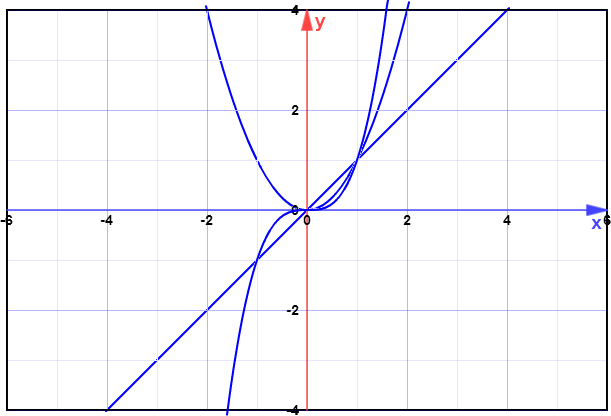
\includegraphics[width=.9\linewidth]{fig_power_function}
\caption{Different power functions.}
\label{fig:power_function}
\end{figure}

\clearpage

\section{Conclusions}

The authors hope that they have acquainted the reader with the concept of motion capture and provided valuable insight into the inner workings of such a framework. We feel that the topics discussed concisely illustrate the issues we were faced with and the manner in which they have been addressed, alongside their advantages and drawbacks. Reflecta aims to become an essential tool for indie game and NUI developers alike. It paves the way for virtually limitless applications in the NUI field of research:

\begin{itemize}
\item Motion capture acquisition and analysis;
\item 3D animation tool-kit;
\item Recovery exercises for patients with motor impairment (see MIRA Rehab \cite{bib_mira} as an example of this type of application);
\item Recovery for patients with psychological disorders (by means of avatar interaction);
\item Intelligent virtual personal assistants (the Cortana from the game HALO may be just around the corner);
\item Party entertainment in pubs/bars - holographic projections of a 3D dancer, with movements streamed from a real person;
\item Virtual reality role playing games (in which one assumes a virtual avatar and interacts with other players);
\end{itemize}

Certainly the list does not end here and we hope to see where development and technology will take us in the not so distant future.

\clearpage

\section{Future work}

Many of the aforementioned algorithms have room for improvement:

\begin{itemize}
\item Noise reduction parameters can be made adaptive to environmental conditions;
\item Extra tracking information from the Kinect can be taken into consideration, such as hand open/closed states and mapped onto Mecanim;
\item Raw animation could be exported to other animation formats for integration into other 3D workflows;
\item Since the Kinect facial expressions are somewhat limited, one could implement custom facial tracking algorithms that analyse the Kinect data stream and provide a wider range of expressions (here, CTRNN or continuous time recurrent neural network models may provide a good starting point);
\item Fully exploit the multi-skeleton tracking of the Kinect sensor to animate an entire crowd of avatars;
\item Explore the possibility of attaching an AI system to Reflecta, enabling it to recognize voice commands and synthesize speech;
\item Fit Reflecta into the much larger context of agent based systems;
\end{itemize}

\clearpage

\section{Acknowledgements}

The author would like to thank Assoc.\ Prof.\ Ph.D.\ Simona Motogna\footnote{motogna@cs.ubbcluj.ro} for her invaluable support as tutor for this dissertation thesis. We also acknowledge that two of our colleagues, Alina Pan\u{a}\footnote{pais0863@scs.ubbcluj.ro} and Ildik\'{o} Szab\'{o}\footnote{siis0870@scs.ubbcluj.ro} have referenced the core functionality of Reflecta in their dissertation work and we appreciate their constructive feedback.

\clearpage

\begin{thebibliography}{10} % Listed in Alphabetical Order

\bibitem{bib_mixamo}
Adobe Systems Inc., Mixamo, A 3D character pipeline built for game devs, \url{https://www.mixamo.com/}.

\bibitem{bib_candide_3}
J. Ahlberg, CANDIDE-3 - An Updated Parameterised Face, Image Coding Group, Dept. of Electrical Engineering, Link\"{o}ping University, 2001.

\bibitem{bib_3ds_max}
Autodesk Inc., 3ds MAX, 3D modeling, animation, and rendering software, \url{http://www.autodesk.com/products/3ds-max/overview}.

\bibitem{bib_maya}
Autodesk Inc., Maya, Comprehensive 3D animation software, \url{http://www.autodesk.com/products/maya/overview}.

\bibitem{bib_blender}
Blender Foundation, Blender, A free and open source 3D creation suite, \url{https://www.blender.org/}.

\bibitem{bib_mira}
A. Cantea, A. C\u{a}lin, A. Dasc\u{a}lu, C. Mihaiu, MIRA Rehab, \url{http://www.mirarehab.com/}.

\bibitem{bib_google_protocol_buffers}
Google Inc., Protocol Buffers, A language-neutral, platform-neutral extensible mechanism for serializing structured data, \url{https://developers.google.com/protocol-buffers/}.

\bibitem{bib_intel_real_sense}
Intel Corporation, Intel RealSense 3D Camera, \url{http://www.intel.com/content/www/us/en/homepage.html}.

\bibitem{bib_motion_capture_editing}
M. Jung, R. Fischer, M. Gleicher, J. Thingvold, M. Bevan, Motion Capture and Editing, A K Peters, 2000.

\bibitem{bib_desp}
J. J. LaViola, Double Exponential Smoothing: An Alternative to Kalman Filter-based Predictive Tracking, Proceedings of the Workshop on Virtual Environments, 2003, p. 199-206.

\bibitem{bib_leap_motion}
Leap Motion Inc., Leap Motion Controller, \url{https://www.leapmotion.com/}.

\bibitem{bib_motion_capture_computer_animation}
A. Menache, Understanding Motion Capture for Computer Animation and Video Games, Morgan Kaufmann, 1999.

\bibitem{bib_motion_capture_explained}
M. Meredith, S. Maddock, Motion Capture File Formats Explained, Technical report CS-01-11, Department of Computer Science, University of Sheffield, 2001.

\bibitem{bib_microsoft_kinect_v1_sdk}
Microsoft Corporation, Kinect for Windows SDK v 1.8, \url{https://msdn.microsoft.com/en-us/library/hh855347.aspx}.

\bibitem{bib_microsoft_kinect_v2_sdk}
Microsoft Corporation, Kinect for Windows SDK v 2.0, \url{https://msdn.microsoft.com/en-us/library/dn799271.aspx}.

\bibitem{bib_msdn}
Microsoft Corporation, MSDN Library - Documentation for developers using Microsoft technologies and tools, \url{http://msdn.microsoft.com/en-us/library}.

\bibitem{bib_mono_game}
MonoGame Team, MonoGame, Write once, play everywhere: One framework for creating powerful cross-platform games, \url{http://www.monogame.net/}.

\bibitem{bib_kalman}
H. Musoff, P. Zarchan, Fundamentals of Kalman Filtering: A Practical Approach, Progress in Astronautics and Aeronautics, Volume 190, American Institute of Aeronautics and Astronautics, 2000.

\bibitem{bib_quaternions}
K. Shoemake, Animating Rotations with Quaternion Curves, Proceedings of SIGGRAPH, ACM Press, 1985, p. 245-254.

\bibitem{bib_poser}
Smith Micro Software Inc., Poser 3D Animation Software, \url{http://my.smithmicro.com/poser-3d-animation-software.html}.

\bibitem{bib_unity}
Unity Technologies Inc., Unity 5 Game Engine, \url{https://unity3d.com/}.

\end{thebibliography}

\clearpage

\listoffigures

% \clearpage

% \listoftables

\end{document}
